\documentclass{article}
\usepackage{lmodern}
\usepackage{amsmath}
\usepackage{graphicx}
\graphicspath{ {img/} }
\usepackage{hyperref}
\hypersetup{
    colorlinks=true,
    linkcolor=blue,
    filecolor=magenta,      
    urlcolor=blue,
}


\title{From Mathematics to Generic Programming}
\author{Brooks Mershon}
\date{April 2017}

\begin{document}

\maketitle

\section*{2.1}


\textit{Solution.}

\bigskip

See Donald Knuth's extensive treatment of this problem starting on \href{http://library.aceondo.net/ebooks/Computer_Science/algorithm-the_art_of_computer_programming-knuth.pdf}{p. 444 (458, PDF) of \textit{The Art of Computer Programming} (Second Edition)}.

Here is a diagram from Knuth with optimal addition chains visualized as a tree for *n* less than 100. The lengths of paths correspond to the length of an optimal addition chain. Note, the problem of finding optimal multiplications for exponentiation happens to be able to be reduced to addition chains, hence the discussion of *multiplication* in Knuth's treatment.

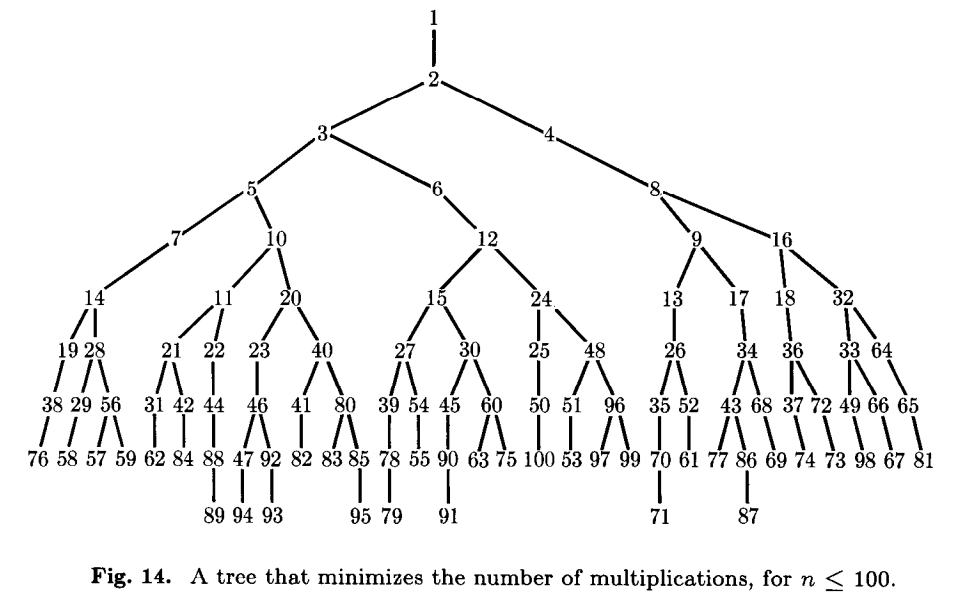
\includegraphics[width=\textwidth]{addition_chains.png}

\end{document}
